\documentclass[addpoints,12pt]{exam}
\newcommand{\ds}{\displaystyle}
\usepackage[margin=0.8in]{geometry}
\usepackage{subcaption}
\usepackage{tikz}
\usepackage{amssymb,amsmath,graphicx,wrapfig,verbatim,wasysym, enumitem,psfragx,color}
\usepackage{multicol}

\usepackage{tikz}
\usepackage{graphicx,ctable,booktabs}

%\usepackage{fancyhdr}
%\setlength{\headheight}{13.6pt}
%\pagestyle{fancy}
%\lhead{Math 222}
%\chead{ Midterm 1 }
%\rhead{Spring 2022}

\def\FillInBlank{\rule{3truein} {.01truein}}


% Choose one option (bubbles)
\newcommand{\chooseone}{{\Large$\Circle$\ \ }}


\newcommand{\myleft}{\makebox[.4\textwidth]{First Name:\enspace\hrulefill}}
\newcommand{\myright}{\makebox[.4\textwidth]{Last Name:\enspace\hrulefill}}
\header{\oddeven{\myleft}{}}
    {}
    {\oddeven{\myright}{}}

\footrule

\footer{Math 211}
     {Final Exam - Practice Exam}
     {Page \thepage\ of \numpages}

\begin{document}

\begin{questions}


\question Are each of the following true or false statements? Fill in the bubble next to the
correct answer. Justification is not necessary.

\begin{parts}


\part[2] If $f(x,y)=\dfrac{\ln(2x)}{y}$, the domain of $f(x,y)$ is $\{(x,y)|x>0, y>0\}.$

\begin{itemize}[label={}]
\item \chooseone True
\item \chooseone False
\end{itemize}

\vfill




\part[2] The improper integral $\ds\int_{9}^\infty \dfrac{4}{x^2}dx$ is divergent.
\begin{itemize}[label={}]
\item \chooseone True
\item \chooseone False
\end{itemize}

\vfill




\part[2] The improper integral $\ds\int_{9}^\infty \dfrac{4}{\sqrt{x}}dx$ is divergent.

\begin{itemize}[label={}]
\item \chooseone True
\item \chooseone False
\end{itemize}

\vfill

\part[2] An equation for the tangent line of $f(x)=2x^3+4x$ at $x=-1$ is $y=10x+4$.

\begin{itemize}[label={}]
\item \chooseone True
\item \chooseone False
\end{itemize}

\vfill


\part[2] The area between the curves $y=\frac{x^2}{4}-2$ and $y=\frac{x}{2}$ (see graph below)
is given by the integral $\ds\int_{-2}^4\left(\frac{x^2}{4}-2-\frac{x}{2}\right)dx$.

\begin{itemize}[label={}]
\item \chooseone True

\item \chooseone False
\end{itemize}

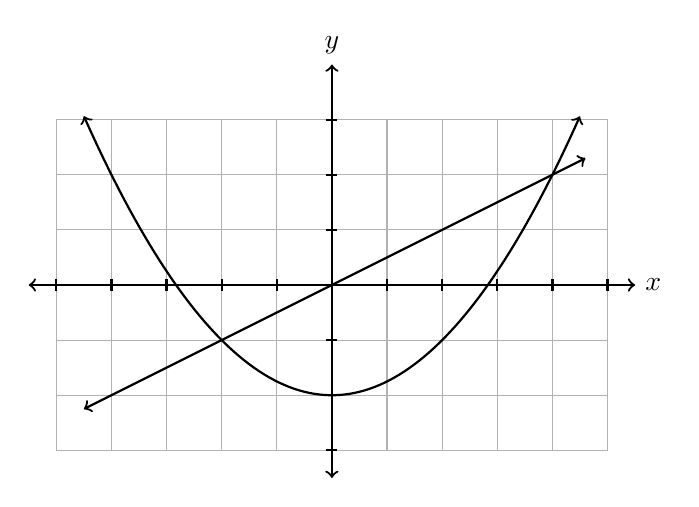
\begin{tikzpicture}[scale=.7]
\draw[gray!60] (-5, -3) grid[step=1] (5, 3);
\draw[<->,thick,black] (-5.5,0)--(5.5,0) node[right]{$x$};
\draw[<->, thick,black] (0,-3.5)--(0,4) node[above]{$y$};
\foreach \x in {-5,-4,...,5}
\draw[thick] (\x,-.1) --(\x,.1);
\foreach \y in {-3,-2,...,3}
\draw[thick] (-.1,\y) --(.1,\y);
\draw[domain=-4.5:4.5,samples=100, thick,<->] plot ({\x},{\x*\x/4-2});
\draw[domain=-4.5:4.6,samples=100,thick,<->] plot ({\x},{\x/2});
\end{tikzpicture}




\vfill


\end{parts}

\newpage


\newpage


\question
Calculate the derivative of each function. You do not need to simplify your answer.


\begin{parts}

\part[4] $f(x)=\ds\frac{1}{2x^4}-\sqrt{3x}+e^2$


\vfill


\part[4] $\ds g(x)=e^{x^2+2x}$

\vfill


\part[5] $F(x)=(3x^4+e^x)^8$

\vfill

\part[5] $r(x)=(4x^3+7x)\ln(x)$

\vfill




\end{parts}

\newpage

%Revenue optimization

\question
Calculate each integral. You do not need to simplify your answer. Show all work.
\begin{parts}

\part[5] $\ds \int \left(10x^4+\dfrac{8}{x}+\dfrac{3}{x^2}\right)dx $

\vspace{1.75in}

\part[6] $\ds \int \sqrt{x}(4x^3+7) dx $

\vfill

\part[6] $\ds \int \left( 4e^{2x} + \dfrac{1}{2} \right)dx $

\vfill

\end{parts}


\newpage

\question[9] A company's marginal cost function is $MC(x)=2e^{-x}$, where $x$ is the number of
units. Find the total cost of producing the first hundred units ($x=0$ to $x=100$). Show all work.
You do not need to simplify your final numerical answer.


\newpage

\question[7] Find the average value of $f(x)=x-3\sqrt{x}$ on the interval $[1,4]$.


\newpage

\question A parking lot owner has $450$ parking spots to rent out. If the owner charges $x$
dollars per parking spot, the number of spots that
will be rented out is given by the function

$$f(x)= 450-10x.$$

\begin{parts}

\part[2] Find $R(x)$, where $R(x)$ is the revenue the parking lot owner receives as a function of
$x$.

\vspace{3in}

\part[5] What price should the parking lot owner charge to maximize revenue? Justify your
solution is optimal. Show all work.

\end{parts}

\newpage




\question
Reminder: If $d(x)$ is the demand function, and $s(x)$ is the supply function,




$(\text{Consumers' surplus for $d(x)$ at demand level $A$})=\ds\int_0^A[d(x)-B]dx$ (where
$B=d(A)$)


$(\text{Producers' surplus for $s(x)$ at demand level $A$})=\ds\int_0^A[B-s(x)]dx$ (where
$B=s(A)$)

\bigskip

Suppose a product has demand function $d(x)=300-\frac{1}{2}x^2$ and supply function
$s(x)=\frac{1}{4}x^2$. %%flip the 1/2 and the 1/4 on the makeup.
\begin{parts}
\part[5] Find the \textbf{producers' surplus} at demand level $A=10$. Show all work. Evaluate
the integral, but you do not need to simplify your final numerical answer.
\vfill
\part[3] Find the \textbf{market demand} (the positive value of $x$ where supply and demand
are equal). Show all work. Simplify your final answer.

\vspace{3in}




\end{parts}
\newpage

\question For $f(x,y)=x^3+y^2-12x+6y$:

\begin{parts}

\part[2] Find the partial derivative $f_x$.

\vspace{2in}

\part[2] Find the partial derivative $f_y$.

\vspace{2in}

\part[4] Find all the critical points of $f(x,y)$. Write each in the form $(x,y)$. Show all work.

\end{parts}

\newpage




\newpage
\question
Use the graph of $y=f'(x)$ to answer the following. {Briefly justify your answers.}

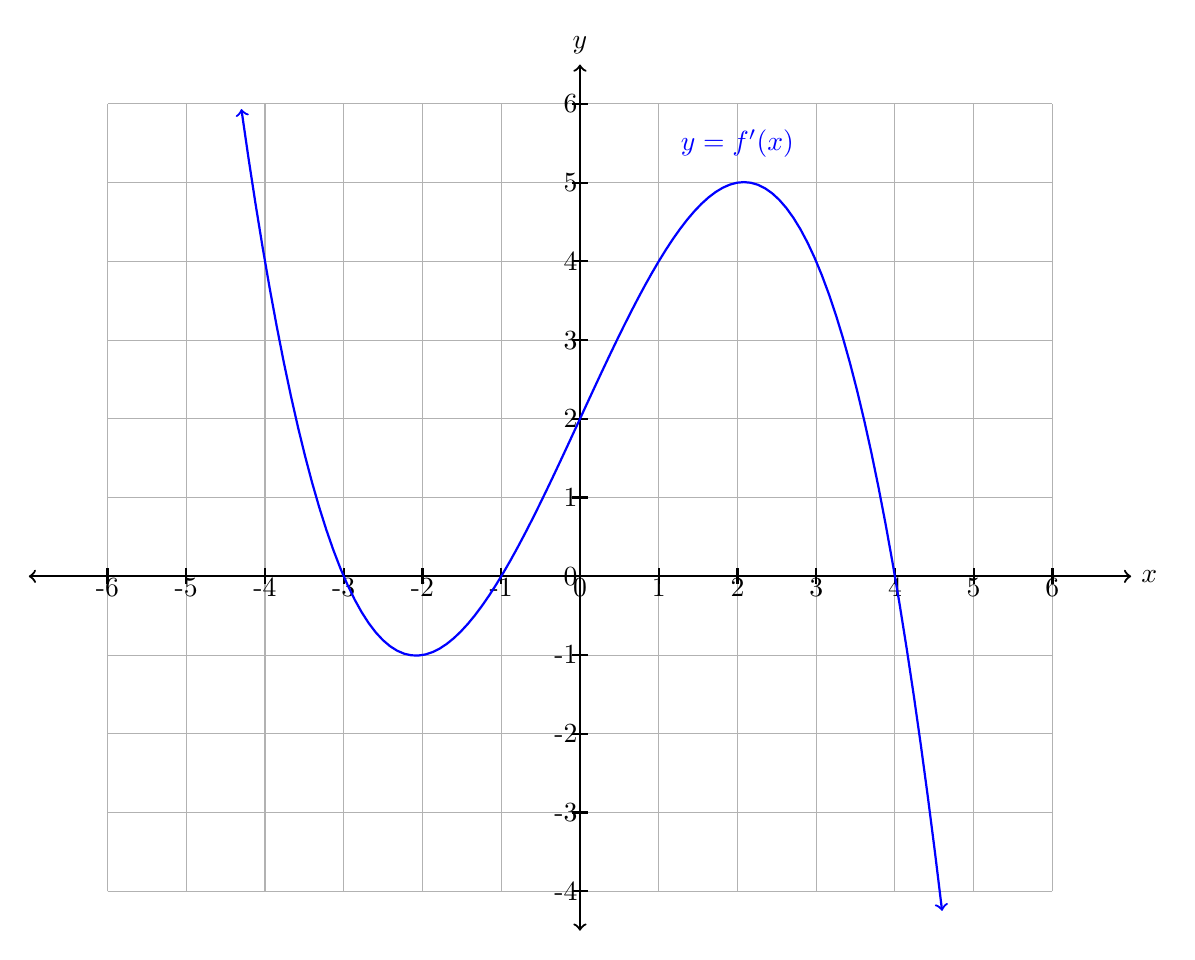
\begin{tikzpicture}[scale=1]
\draw[gray!60] (-6, -4) grid[step=1] (6, 6);
\draw[<->,thick,black] (-7,0)--(7,0) node[right]{$x$};
\draw[<->, thick,black] (0,-4.5)--(0,6.5) node[above]{$y$};
\foreach \x in {-6,-5,...,6}
\draw[thick] (\x,-.1) --(\x,.1) node[below] { \x};
\foreach \y in {-4,-3,...,6}
\draw[thick] (-.1,\y) --(.1,\y) node[left] { \y};
\draw[domain=-4.3:4.6,samples=100, thick,<->,color=blue] plot ({\x},{-(\x+1)/6*(\x+3)*(\x-4)});
\node[color=blue] at (2,5.5) {$y=f'(x)$};
\end{tikzpicture}

Again, \textbf{this is the graph of the derivative of $f(x)$.}
\begin{parts}
       \part[2] On which interval(s) is $f(x)$ increasing? Briefly justify your answer.
 \vfill

         \part[2] Is $f(x)$ concave up or concave down at $x=-4$? Briefly justify your answer.
 \vfill

       \part[2] What is $\displaystyle \lim_{h\to0}\frac{f(3+h)-f(3)}{h}$? Briefly justify your
answer.
 \vfill

 \end{parts}


\newpage

\question For the function $f(x,y)=x^3-y^3-9xy+4$:
\begin{parts}
\part[5] Compute $f_{xx}, f_{yy},$ and $f_{xy}$. Show all work.
\vspace{3in}


\part[5] The critical points of $f(x,y)$ are $(0,0)$ and $(-3,3)$. Determine, using the $D$-test, if
each point corresponds to a relative maximum, relative minimum, or saddle point. Show all
work.

Reminder: $D=f_{xx}(a,b)f_{yy}(a,b)-[f_{xy}(a,b)]^2$

\end{parts}
\vspace{0.25in}

\newpage




\newpage




\end{questions}

\end{document}
